%%%%%%%%%%%%%%%%%%%%%%%%%%%%%%%

%\fixme{KM: done for now, but am not satisfied with the end of it-- Juergen did not provide measurements! SG/JM: please briefly check to make sure it is coherent? SG: done. Sent an email to Juergen with some items to be addressed.}

\subsubsection{Physics Motivation}

Radioactive source deployment provides an in-situ source of physics signals at a known location and with a known activity that can be chosen such that there is only one calibration event per drift time window. The baseline source design probes de-excitation products (gamma-rays) which are directly relevant for detection of supernova neutrinos and/or $^{8}B$ solar neutrinos. Secondary measurements from the baseline source deployment include electro-magnetic (EM) shower characterization for long-baseline $\nu_e$ CC events, electron lifetime as a function of  \dword{detmodule} vertical position, trigger efficiency study versus threshold, and help determine radiative components of the Michel electron energy spectrum from muon decays. Aside from the baseline source, other sources could be deployed with the same multi-purpose system that probe for example the impact of various radiological backgrounds or measure the neutron tagging efficiency, useful for improved calorimetry of beam neutrino interactions.

Both the radioactive source system and the pulsed neutron source system are needed to address integrated response of the detector for low energy physics. Response in Ar may change rapidly as a function of photon energy due to underlying nuclear physics mechanisms. A combination of 6 MeV (direct neutron capture response), 9 MeV (peak visible $\gamma$-energy of interest to \dword{snb}), and decay electrons (~30 MeV) is needed to map this response. In terms of complementarity, radioactive sources provide a known position, known-energy single photon events while the pulsed neutron source provides a simple, potentially, non-invasive design with multi-photon energy signature which is visible across the entire detector with a known time signature.


%%%%%%%%%%%%%%%%
\subsubsection{Design Considerations}

A composite source can be used that consists  of $^{252}$Cf, a strong neutron emitter, and $^{58}$Ni, which, via the $^{58}$Ni(n,$\gamma$)$^{59}$Ni process, converts one of the $^{252}$Cf fission neutrons, suitably moderated, to a monoenergetic \SI{9}{\MeV} photon~\cite{Rogers:1996ks}. 
The source is envisaged to be inside a cylindrical moderator with mass of about \SI{15}{kg} and a diameter of \SI{20}{\cm} such that it can be deployed via the multipurpose instrumentation ports discussed in Section~\ref{sec:calib-ports}. The activity of the radioactive source is chosen such that no more than one \SI{9}{\MeV} capture $\gamma$-event occurs during a single 
drift period. This allows one to use the arrival time of the measured light as a $t0$ and then measure the average drift time of the corresponding charge signal(s). The sources would be deployed outside the \dword{fc} within the cryostat to avoid regions with a high electric field, about \SI{30}{\cm} from the field cage. The $\gamma$-ray would need
to travel about two attenuation lengths (including the \SI{10}{\cm} radius of the source body). Such high
$\gamma$-energies are typically only achieved by thermal neutron
capture, which invokes a neutron source surrounded by a large
amount of moderator,
thus making such an externally deployed (n, $\gamma$) source \SI{20}{\cm}  to \SI{50}{\cm} % large
in diameter. 

In Ref.~\cite{Rogers:1996ks},
%\cite{Triumf:Nickelsource} 
%\todo{SG: reference needs fixing},
a $^{58}$Ni (n,$\gamma$) source, triggered by an AmBe neutron source,
was successfully built, yielding high $\gamma$-energies of \SI{9}{\MeV}. DUNE %We
proposes to use a $^{252}$Cf (or AmLi as backup) neutron source with lower
neutron energies, which requires less than half of the surrounding
moderator, and making the $^{58}$Ni (n, $\gamma$) source only
\SI{20}{\cm} or less in diameter. The multipurpose instrumentation
feedthroughs at either end of the cryostat are sufficient for
this, and have an inner diameter of \SI{25}{\cm}.  The moderator
material chosen for DUNE is Delrin which has a large enough
density to avoid flotation. Further, the end caps of the source
body are round to avoid distorting the electric field and to
eliminate the risk of the source getting stuck during deployment. 
Figure~\ref{fig:RadSource} depicts the baseline source design of a
cylindrical Delrin moderator with a diameter of \SI{20}{\cm}, a
height of \SI{40}{\cm} including half-spheres at either end with
radius of \SI{10}{\cm}, deployed at $z$=\SI{40}{\cm} leaving a gap of \SI{30}{\cm} towards the \dword{fc} and at a distance to the \dword{apa} of $x$=\SI{220}{\cm}, 
which is slightly further than mid-drift.

\begin{dunefigure}[h]{fig:RadSource}{Fish-line deployment scheme in DUNE for a radioactive source
encapsulated inside a cylindrical Delrin moderator body with a
diameter of \SI{20}{\cm}, a height of \SI{40}{\cm} including
half-spheres at either end with radius of \SI{10}{\cm}. A
$^{252}$Cf neutron source and a natural nickel target are sealed
inside at the center. The fish-line is deployed \SI{40}{\cm}
outside of the \dword{fc} and at \SI{220}{\cm} distance to the
\dword{apa} (red plane).}
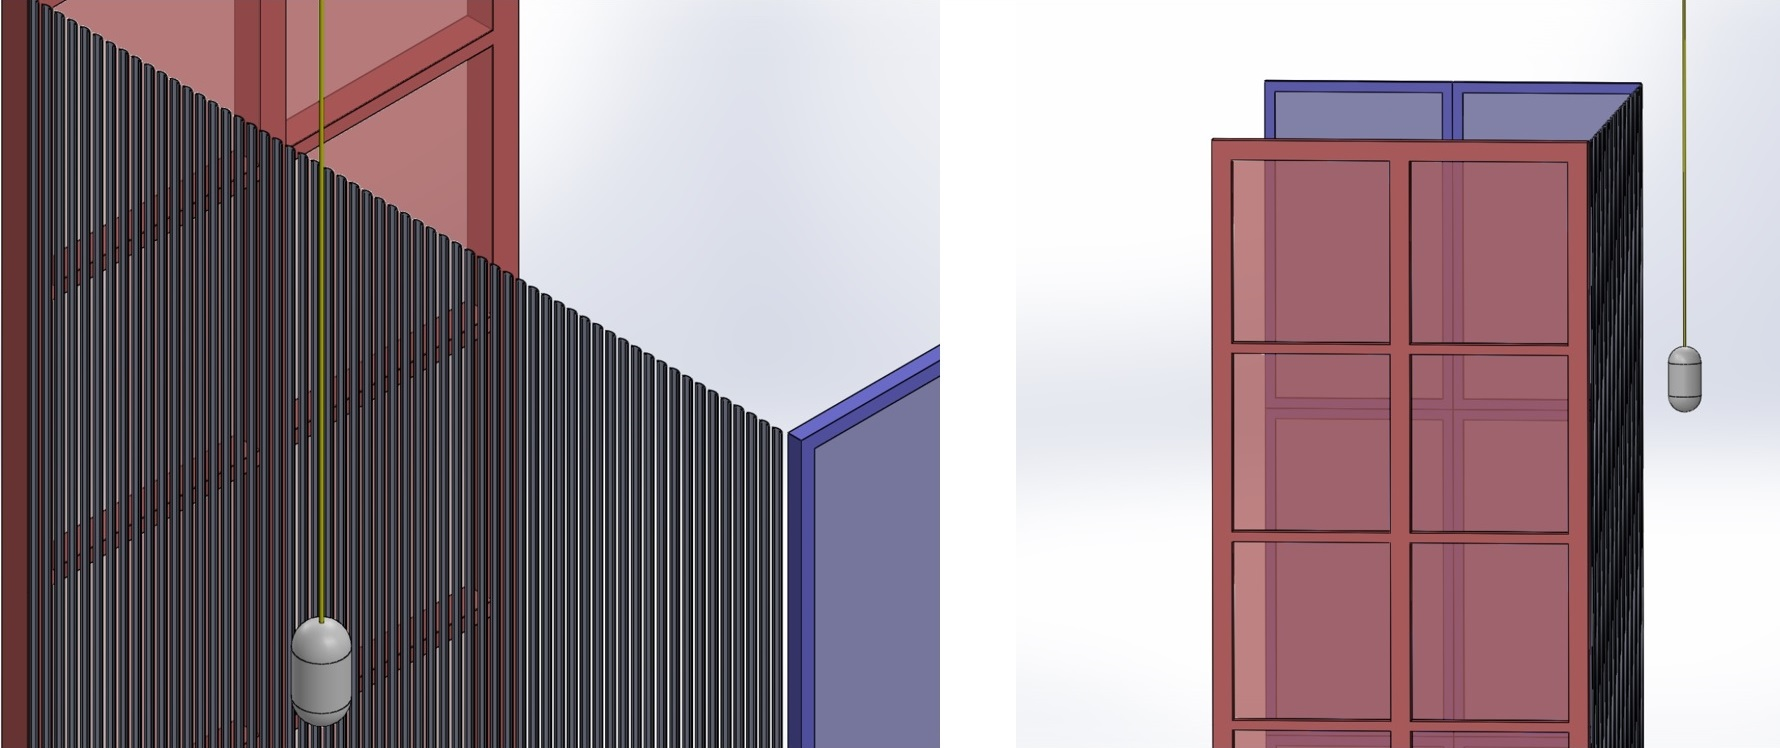
\includegraphics[width=1.0\linewidth]{RadioactiveSource_zm40cm_xp220cm.jpg}
\end{dunefigure}

% Here it is, but I don't have privileges for the bibliography

%@Misc{Triumf:Nickelsource,
%  author =   {J. Rogers, M. Andreaco, C. Moisan},
%  title =    {A $7-9$\,MeV isotropic gamma ray source for detector testing},
%  howpublished = {TRIUMF TRI-PP-96-7},
%  month =    {Apr},
%  year =     {1996},
%}

%\fixme{KM: From Juergen but I think covered by above: The activity of the radioactive source is chosen such that no more than one \SI{9}{\MeV} capture $\gamma$-ray spills into the active \dword{lartpc} region during a single \SI{2.2}{\milli\s} drift period. This allows one to use the arrival time of the measured light as $t_{0}$ and then measure the average drift time of the corresponding charge signal(s). The resulting drift velocity in turn yields the electric field strength, averaged over the variations encountered during the drifting of the charge(s). This can be repeated for each single \SI{9}{\MeV} capture $\gamma$-event that occurs during a \SI{2.2}{\milli\s} drift period and where visible $\gamma$-energy is deposited inside the active volume of the TPC. Pile-up and data read-out considerations restrict the maximally permissible event rate to less than \SI{10}{\hertz} and in turn the \SI{9}{\MeV} capture $\gamma$-rate occurring inside the radioactive source body to less than \SI{140}{\hertz}, given a spill-in efficiency into the active \dword{lar} of about \num{7}\%.}

A successfully employed multipurpose fish-line calibration
system~\cite{DCnearDetTDR} \todo{SG: Juergen to provide proper reference.} 
%\fixme{need to add reference: "The Double Chooz Near Detector Technical Design Report" 
%Double Chooz Collaboration (H. de Kerret (APC, Paris) et al.) Oct 1, 2012. EDMS ID:I-028812 ; DocDB ID: 3403-V5 Pages 198 - 223
%(Anne can't find proper ref for this)}
 for the Double Chooz
reactor neutrino experiment has become available for DUNE after
the decommissioning of Double Chooz in 2018. The system can be
easily refitted for use in DUNE. The system will be housed inside
a purge-box that is connected via a neck to a multipurpose
calibration feedthrough with a closed gate valve on top of the
cryostat. Before deployments, the purge-box will be evacuated by a
vacuum pump, then purged with argon gas, and the pressure
equalized with the gas pressure inside the detector, before the
gate-valve is opened and deployments can commence. 
%Also, if the source is in close proximity of an \dword{apa} wire frame, lower energetic radiological backgrounds become problematic as the source light and charge yield is reduced exponentially with distance. 
Near mid-drift (in each TPC module) the \SI{9}{\MeV}
$\gamma$-ray source can illuminate the full drift length from
\dword{apa} to \dword{cpa}. The sources are retrieved from the
detector after each deployment and stored outside the cryostat following approved safety protocols.

The commissioning plan for the source deployment system will include a dummy 
source deployment (within 2 months of the commissioning) followed by first real source deployment (within 3-4 months of the commissioning) and a second real source deployment (within 6 months of the commissioning). Assuming stable detector conditions, the radioactive source will be deployed every half a year. Ideally, a deployment before and after a run period are desired so at least two data points are available for calibration. This also provides a check if the state of the system
has changed before and after the physics data run.
%If stability fluctuates for any reason (e.g., electronic response changes over time) at a particular location, one would want to deploy the source at that location once a month, or more often, depending on how bad the stability is.
It is expected that it will take a few hours (e.g. 8 hours) to deploy the system at one feedthrough location and a full radioactive source calibration campaign might take %at least 
a week.

The major development plans for the radioactive source system include:
\begin{itemize}
\item Continued development of relevant simulation tools including geometry representation of the source deployment system, impact from various radiological contaminants on detector response. 
\item Studies to suppress radiological backgrounds for the calibration source
\item Simulation studies to understand data and trigger rates;
\item Build a baseline design source with Delrin moderator, $^{252}$Cf neutron source and natural nickel target, both sealed inside at the moderator's center.
\item Validate \SI{9}{\MeV} capture $\gamma$-ray yield of source by spectroscopic measurements with a germanium detector (that also has a large enough assay chamber) at South Dakota School of Mines and Technology.
\item Validate with $^{3}$He based hodoscope at South Dakota School of Mines and Technology that the flux of neutrons escaping from the moderator is not an issue (otherwise use lower energetic AmLi neutron source instead and/or more moderator material, and/or different geometric configuration of nickel target). 
\item Validate that anticipated fluid flow in \dword{lar} does not cause oscillations of the source (otherwise design vertical guide wires that will get pre-installed during detector installation and that will keep source stable in position during a deployment along the vertical axis).
\item A mechanical test of the Double Chooz fish-line deployment system with a \dword{lar} (and liquid nitrogen) mock-up column will be done in the high bay lab at South Dakota School of Mines and Technology. The ultimate test of the system will be done at ProtoDUNE. 
\item Other radioactive sources beyond the baseline design will be explored that will help understand the impact of various radiological backgrounds such as e.g. hybrid neutron sources ($^{252}$Cf and AmBe) that emulate the kinetic neutron energy spectrum of radiological neutrons and probe the neutron tagging efficiency.
\end{itemize}

A successful demonstration of the radioactive source system in ProtoDUNE-SP-II running is the main priority for this system towards making a decision on deploying this system for the \dword{fd}. A schedule with main steps towards ProtoDUNE deployment is shown in table~\ref{tab:calib-rsds-sched}.

\begin{dunetable}
[Key milestones towards commissioning the radioactive source deployment system (RSDS) in ProtoDUNE-SP-II.]
{p{0.65\textwidth}p{0.25\textwidth}}
{tab:calib-rsds-sched}
{Key milestones towards commissioning the radioactive source system in ProtoDUNE-SP-II.}  
Milestone & Date (Month YYYY)   \\ \toprowrule
Baseline RSDS design validation & January 2020 \\ \colhline 
RSDS mock-up deployment test at SDSMT & March 2020 \\ \colhline 
RSDS Design review  & May 2020 \\ \colhline
RSDS Production readiness review (PRR) & July 2020 \\ \colhline
Start of module 0 RSDS component production for ProtoDUNE-II & September 2020      \\ \colhline
End of module 0 RSDS component production for ProtoDUNE-II &  February 2021    \\ \colhline
\textbf{Start of ProtoDUNE-SP-II installation} & \textbf{March 2021} \\ \colhline
Start of RSDS installation &  April 2021    \\ \colhline
RSDS demonstration test at ProtoDUNE-SP-II  & April 2022\\ \colhline
\end{dunetable}



%%%%%%%%%%%%%%%%%%%%%%%%%%%%
\subsubsubsection{Possible Measurements}
\label{sec:sp-calib-sys-src-dep-meas}

The 9 MeV single gamma source may also be used to test the gamma aspect of the \dword{snb} signal along the full drift but only in the endwall regions of the detector. The source may also be used to determine the relative efficiency in the vertical direction for measurements of energy resolution and energy scale. Simulation studies are currently underway and for the second draft, we plan to include a first round of simulation results.

%\todo{Simulation studies are underway; for v2 we will include a first round of studies.}